% coding:utf-8

% Ausführen in R: 
% Sweave("C:/Daten/Daniel/studium/git_repo/sem2/stoc/sw07/sw07_4.Rnw",encoding='UTF-8')

\section{Aufgabe 4}

\subsection{a}
\begin{Schunk}
\begin{Sinput}
> plot(seq(0,100,by=0.001),dnorm(seq(0,100,by=0.001),mean=32,sd=6),type='l')
> abline(v=26)
> abline(v=38)
\end{Sinput}
\end{Schunk}
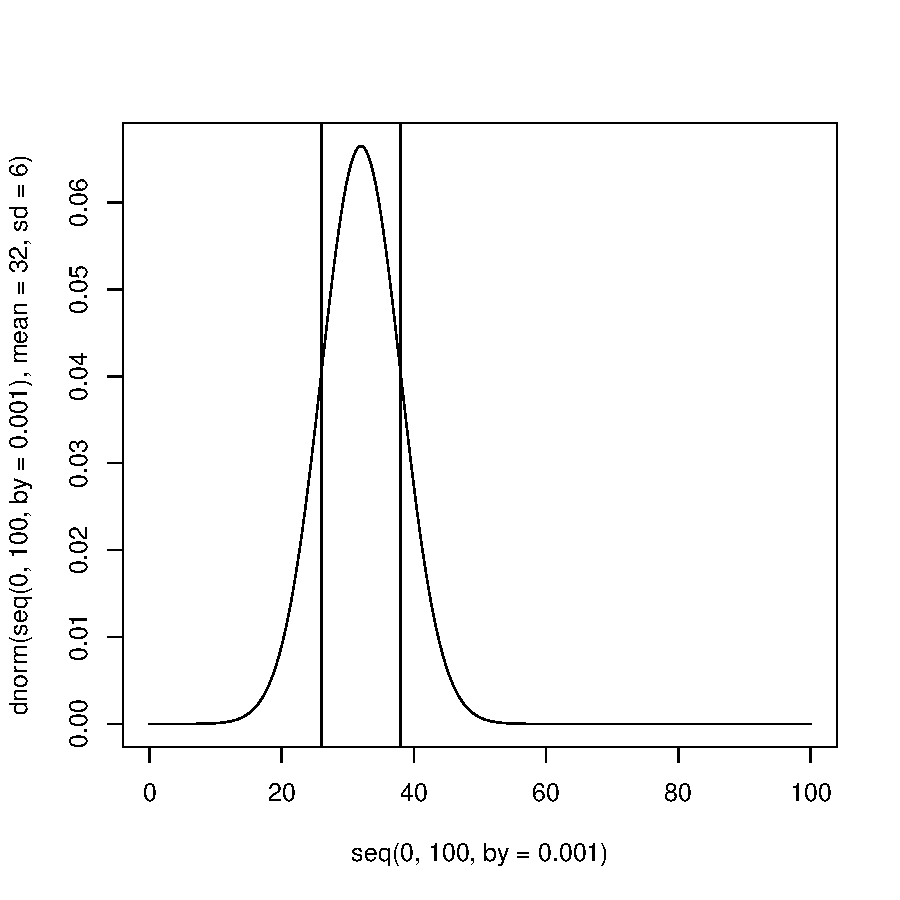
\includegraphics{sw07_4-001}

\subsection{b}
\begin{Schunk}
\begin{Sinput}
> pnorm(40,mean=32,sd=6)
\end{Sinput}
\begin{Soutput}
[1] 0.9087888
\end{Soutput}
\end{Schunk}

\subsection{c}
\begin{Schunk}
\begin{Sinput}
> pnorm(27,mean=32,sd=6)
\end{Sinput}
\begin{Soutput}
[1] 0.2023284
\end{Soutput}
\end{Schunk}

\subsection{d}
% Ausprobiert: 43.75978
\begin{Schunk}
\begin{Sinput}
> qnorm(0.975,mean=32,sd=6)
\end{Sinput}
\begin{Soutput}
[1] 43.75978
\end{Soutput}
\end{Schunk}

\subsection{e}
% Ausprobiert: 24.310692
\begin{Schunk}
\begin{Sinput}
> qnorm(0.1,mean=32,sd=6)
\end{Sinput}
\begin{Soutput}
[1] 24.31069
\end{Soutput}
\end{Schunk}

\subsection{f}
\begin{Schunk}
\begin{Sinput}
> pnorm(38,mean=32,sd=6)-pnorm(26,mean=32,sd=6)
\end{Sinput}
\begin{Soutput}
[1] 0.6826895
\end{Soutput}
\end{Schunk}
